%%%%%%%%%%%%%%%%%%%%%%%%%%%%%%%%%%%%%%%%%%%%%%%%%%%%%%
% Thanks to Xu Minghao's work                        %
% I modify it into uchicago version                  %
% to not make new bug, I don't alter "Ritsumeikan"   %
% keywords in file. Pls feel free to use             %
%%%%%%%%%%%%%%%%%%%%%%%%%%%%%%%%%%%%%%%%%%%%%%%%%%%%%%

%%%%%%%%%%%%%%%%%%%%%%%%%%%%%%%%%%%%%%%%%%%%%%%%%%%%%%
% A Beamer template for Ritsumeikan University       %
% Author: Ming-Hao Xu (Xu Minghao)                   %
% Date:   April 2022.                                %
% LPPL Licensed.                                     %
%%%%%%%%%%%%%%%%%%%%%%%%%%%%%%%%%%%%%%%%%%%%%%%%%%%%%%

\documentclass[handout]{beamer}
\usepackage{hyperref}
\usepackage{lmodern}
\usepackage[T1]{fontenc}

% other packages
\usepackage{latexsym,amsmath,xcolor,multicol,booktabs,calligra}
\usepackage{graphicx,pstricks,listings,stackengine}
\usepackage{wrapfig}
\usepackage{caption}
\usepackage{animate}

\captionsetup[figure]{justification=centering}

\author[Gustavo Quilca]{Jose Gustavo Quilca Vilcapoma
\\
\small Tutor: Javier Alcaraz Soria}

\title{Optimización del Llenado Manual de Contenedores con Paquetes Heterogéneos}
\subtitle{Máster Universitario en Estadística Computacional y Ciencia de Datos para la Toma de Decisiones}
\institute[CIO - UMH]{
    Instituto Centro de Investigación Operativa \\
    Universidad Miguel Hernández
}
\date{\small 17 Junio 2024}
\usepackage{Ritsumeikan}

% defs
\def\cmd#1{\texttt{\color{red}\footnotesize $\backslash$#1}}
\def\env#1{\texttt{\color{blue}\footnotesize #1}}
\definecolor{deepblue}{rgb}{0,0,0.5}
\definecolor{deepred}{RGB}{160,58,56}
\definecolor{deepgreen}{rgb}{0,0.5,0}
\definecolor{halfgray}{gray}{0.55}

\lstset{
    basicstyle=\ttfamily\small,
    keywordstyle=\bfseries\color{deepblue},
    emphstyle=\ttfamily\color{deepred},    % Custom highlighting style
    stringstyle=\color{deepgreen},
    numbers=left,
    numberstyle=\small\color{halfgray},
    rulesepcolor=\color{red!20!green!20!blue!20},
    frame=shadowbox,
}


\begin{document}

\begin{frame}
    \titlepage
    \vspace*{-0.6cm}
    \begin{figure}[htpb]
        \begin{center}
            
\includegraphics[keepaspectratio, scale=0.04]{pic/logos.png}
        \end{center}
    \end{figure}
\end{frame}

\begin{frame}
    \tableofcontents[sectionstyle=show,
        subsectionstyle=show/shaded/hide,
        subsubsectionstyle=show/shaded/hide]
\end{frame}

\section{Introducción}

\begin{frame}{Introducción}
    \begin{itemize}[<+-| alert@+>] % stepwise alerts
        \item El problema del llenado de contenedores (CLP) es un
              problema clásico en la optimización combinatoria.
        \item Consiste en encontrar la mejor manera de llenar un contenedor con paquetes de diferentes tamaños y pesos, optimizando la utilización del espacio.
        \item Este problema tiene aplicaciones en logística, transporte,
              almacenamiento, entre otros.
    \end{itemize}
\end{frame}

\begin{frame}{Restricciones}
    \begin{itemize}[<+-| alert@+>]
        \item Restricciones Básicas
              \begin{itemize}
                  \item No superposición de paquetes.
                  \item No superar el peso máximo del contenedor.
                  \item Colocación dentro de los límites del contenedor.
              \end{itemize}
        \item Restricciones Prácticas
              \begin{itemize}
                  \item Estabilidad de los paquetes.
                  \item Centro de gravedad del contenedor.
                  \item Prioridad de carga.
                  \item Restricción de contigüidad de tipos.
              \end{itemize}
    \end{itemize}
\end{frame}

\begin{frame}{Métodos de Solución}
    \begin{itemize}[<+-| alert@+>]
        \item \textbf{Métodos exactos}:
              \begin{itemize}
                  \item Garantizan la solución óptima, pero son computacionalmente costosos.
              \end{itemize}
        \item \textbf{Métodos heurísticos}:
              \begin{itemize}
                  \item Proporcionan soluciones de buena calidad en un tiempo razonable.
              \end{itemize}
        \item \textbf{Métodos metaheurísticos}:
              \begin{itemize}
                  \item Estrategias flexibles de alto nivel para desarrollar algoritmos que resuelven problemas específicos.
              \end{itemize}
    \end{itemize}
\end{frame}

\section{Problema}

\begin{frame}{Contexto del Problema}
    \begin{itemize}[<+-| alert@+>]
        \item Empresa en el sector de envío de paquetes en contenedores marítimos.
        \item No tiene control sobre las medidas de los paquetes.
        \item Cuenta con una cantidad máxima de paquetes de cada tipo.
        \item Envía un solo contenedor a la vez.
        \item Usan procedimientos establecidos de llenado manual.
    \end{itemize}
\end{frame}

\begin{frame}{Definición del Problema}
    \begin{itemize}[<+-| alert@+>]
        \item Maximizar el beneficio de la carga en un contenedor, con los paquetes disponibles.
        \item Los paquetes apilados deben mantener su estabilidad durante la carga.
        \item Todos los paquetes del mismo tipo son cargados de forma contigua.
        \item Los paquetes del mismo tipo son rotados en una misma dirección.
    \end{itemize}
\end{frame}

\begin{frame}{Definición Formal}
    \begin{columns}
        \begin{column}{0.7\textwidth}
            \begin{center}
                Optimizar la carga de un contenedor, determinando el \textbf{\textcolor{ritsumeikan}{orden}}, la \textbf{\textcolor{ritsumeikan}{cantidad}} y  \textbf{\textcolor{ritsumeikan}{rotación}} de los tipos de paquetes, cumpliendo con las restricciones prácticas del \textbf{\textcolor{ritsumeikan}{llenado manual}}. El objetivo principal es maximizar el beneficio total de la carga.
            \end{center}
        \end{column}
        \begin{column}{0.4\textwidth}
            \begin{figure}
                \centering
                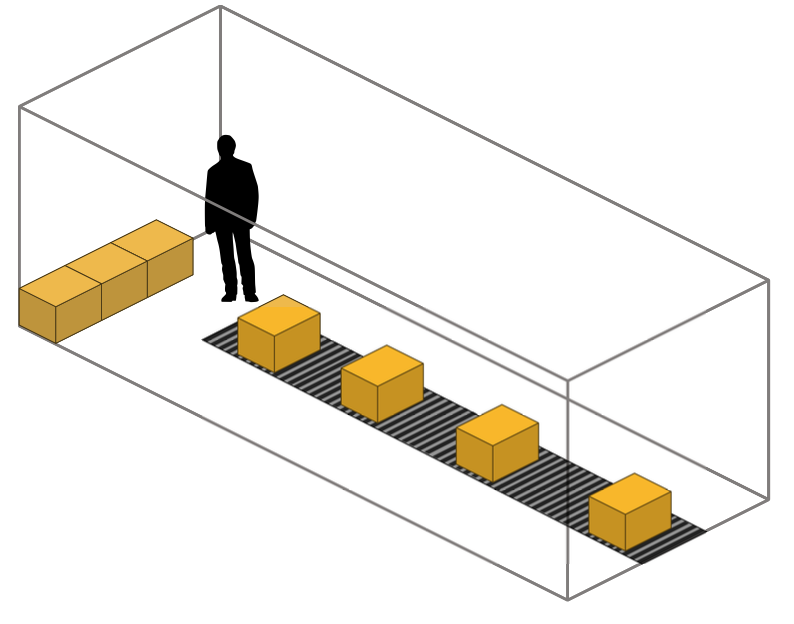
\includegraphics[width=0.95\textwidth]{pic/cinta-transportadora.png}
                \label{fig:cinta-transportadora}
            \end{figure}
        \end{column}
    \end{columns}

\end{frame}

\section{Algoritmo Genético}

\begin{frame}{Algoritmo Genético}
    \begin{columns}
        \begin{column}{0.7\textwidth}
            \begin{exampleblock}{Es una técnica de optimización inspirada en la evolución natural:}
                \begin{enumerate}[<+-| alert@+>]
                    \item Generación y evaluación de una población inicial.
                    \item Selección de los mejores individuos.
                    \item Cruce de los individuos seleccionados.
                    \item Mutación de los individuos resultantes.
                    \item Evaluación y reemplazo de la nueva población.
                    \item Repetir hasta cumplir un criterio de parada.
                \end{enumerate}
            \end{exampleblock}
        \end{column}
        \begin{column}{0.4\textwidth}
            \begin{figure}
                \centering
                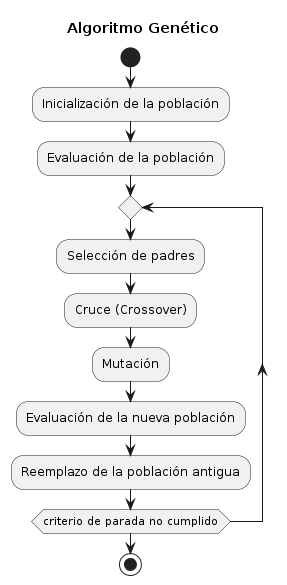
\includegraphics[width=0.75\textwidth]{pic/algoritmo-genetico.png}
                \label{fig:algoritmo-genetico}
            \end{figure}
        \end{column}
    \end{columns}
\end{frame}

\begin{frame}{Algoritmo Genético}
    \begin{columns}
        \begin{column}{0.6\textwidth}
            \begin{exampleblock}{Diseño de la Codificación de las Soluciones:}
                \begin{itemize}[<+-| alert@+>]
                    \item Uso de 3 listas para representar el orden de llenado.
                    \item Ayuda a garantizar factibilidad.
                    \item Es la forma en la que llegarían los paquetes al operario.
                \end{itemize}
            \end{exampleblock}
        \end{column}
        \begin{column}{0.4\textwidth}
            \begin{figure}
                \centering
                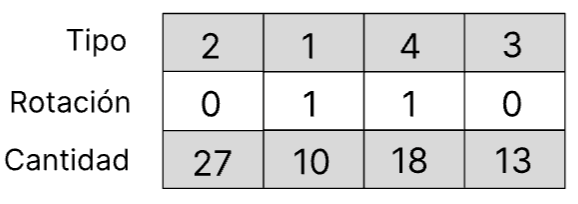
\includegraphics[width=1\textwidth]{pic/codificacion.png}
                \caption*{Ejemplo de codificación}
                \label{fig:codificacion}
            \end{figure}
        \end{column}
    \end{columns}
\end{frame}

\begin{frame}{Algoritmo Genético}
    \begin{exampleblock}{Función de evaluación:}
        \begin{itemize}[<+-| alert@+>]
            \item Calcula el beneficio total de la carga.
            \item Verificar la factibilidad de la soluciones.
            \item Es necesario el desarrollo de un algoritmo que \textbf{imite el procedimiento de llenado manual}.
        \end{itemize}
    \end{exampleblock}
\end{frame}

\begin{frame}{Algoritmo Genético: Función de evaluación}
    \begin{exampleblock}{Algoritmo de llenado manual:}
        Basado en un método conocido como Deepest Bottom Left with Fill (DBLF).
        \begin{figure}
            \centering
            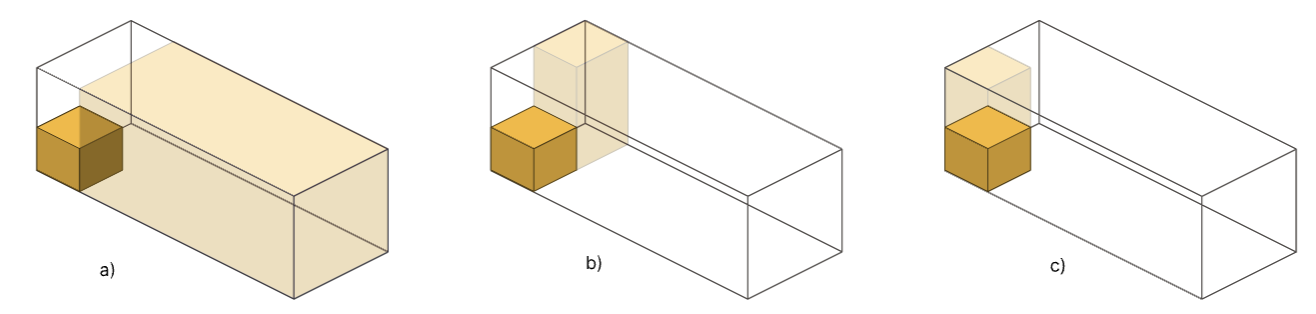
\includegraphics[width=1\textwidth]{pic/dblf.png}
            \caption*{División del espacio restante en el contenedor luego de colocar un paquete}
            \label{fig:dblf}
        \end{figure}
    \end{exampleblock}
\end{frame}


\begin{frame}{Algoritmo Genético: Función de evaluación}
    \begin{columns}
        \begin{column}{0.5\textwidth}
            \begin{exampleblock}{Adaptación del Algoritmo DBLF:}
                \begin{itemize}[<+-| alert@+>]
                    \item Unión de subespacios
                    \item Eliminación de subespacios inaccesibles
                    \item Eliminación de subespacios profundos
                \end{itemize}
            \end{exampleblock}
        \end{column}
        \begin{column}{0.5\textwidth}
            \begin{overlayarea}{\textwidth}{\textheight}
                \visible<1->{
                    \begin{figure}
                        \centering
                        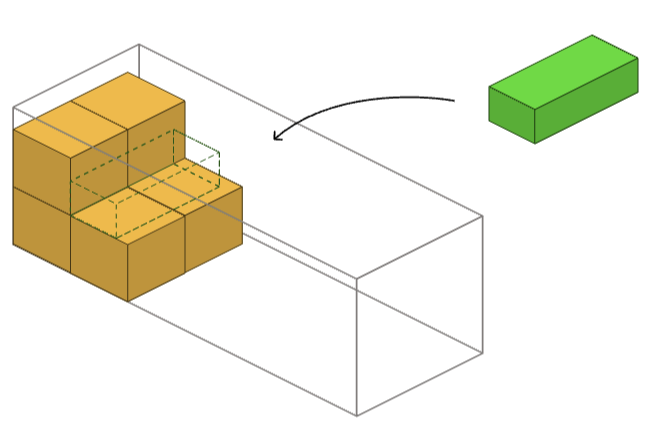
\includegraphics[width=0.7\textwidth]{pic/dblf-adaptado1.png}
                    \end{figure}
                }
                \visible<2->{
                    \begin{figure}
                        \centering
                        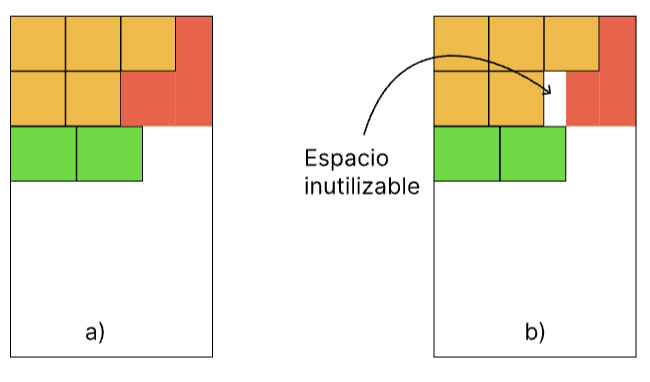
\includegraphics[width=0.5\textwidth]{pic/dblf-adaptado2.png}
                    \end{figure}
                }
                \visible<3->{
                    \begin{figure}
                        \centering
                        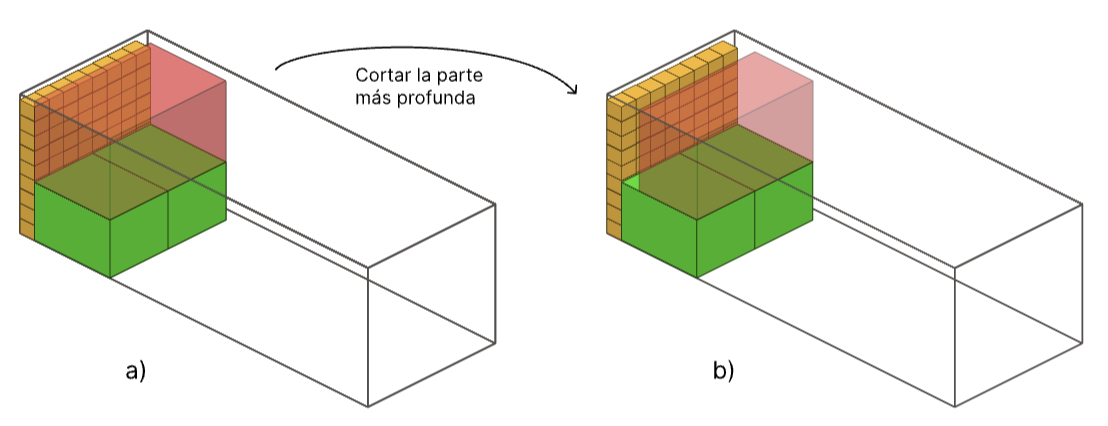
\includegraphics[width=0.75\textwidth]{pic/dblf-adaptado3.png}
                    \end{figure}
                }
            \end{overlayarea}
        \end{column}
    \end{columns}
\end{frame}

\begin{frame}{Algoritmo Genético: Función de evaluación}
    \begin{exampleblock}{Algoritmos adaptados}
        \begin{figure}
            \centering
            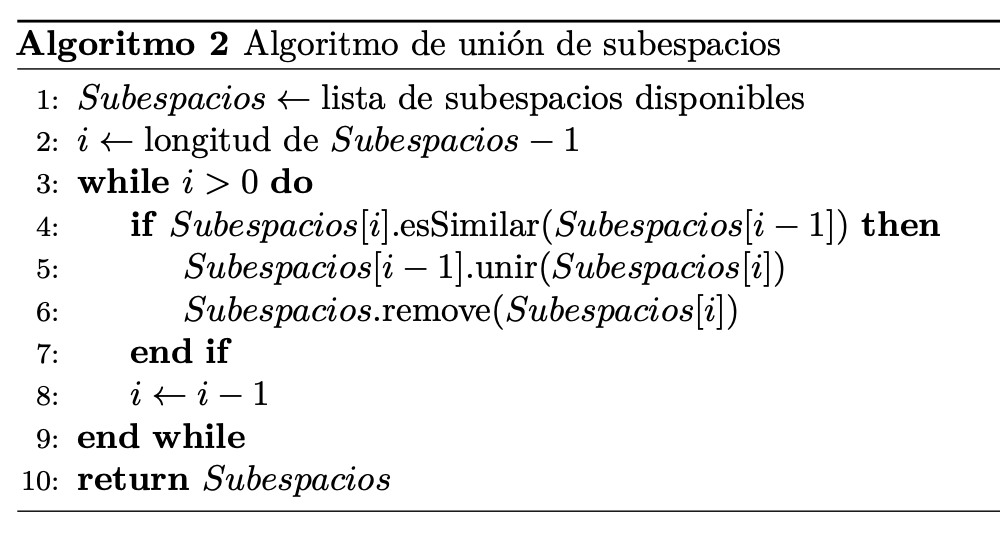
\includegraphics[width=0.48\textwidth]{pic/union-subespacios.png}
            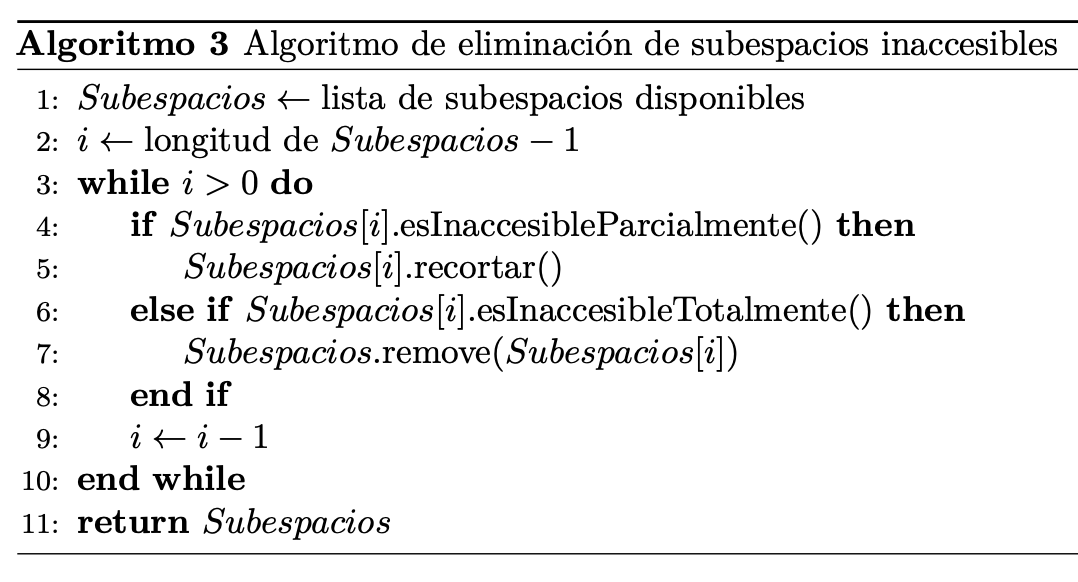
\includegraphics[width=0.48\textwidth]{pic/subespacios-inaccesibles.png}
            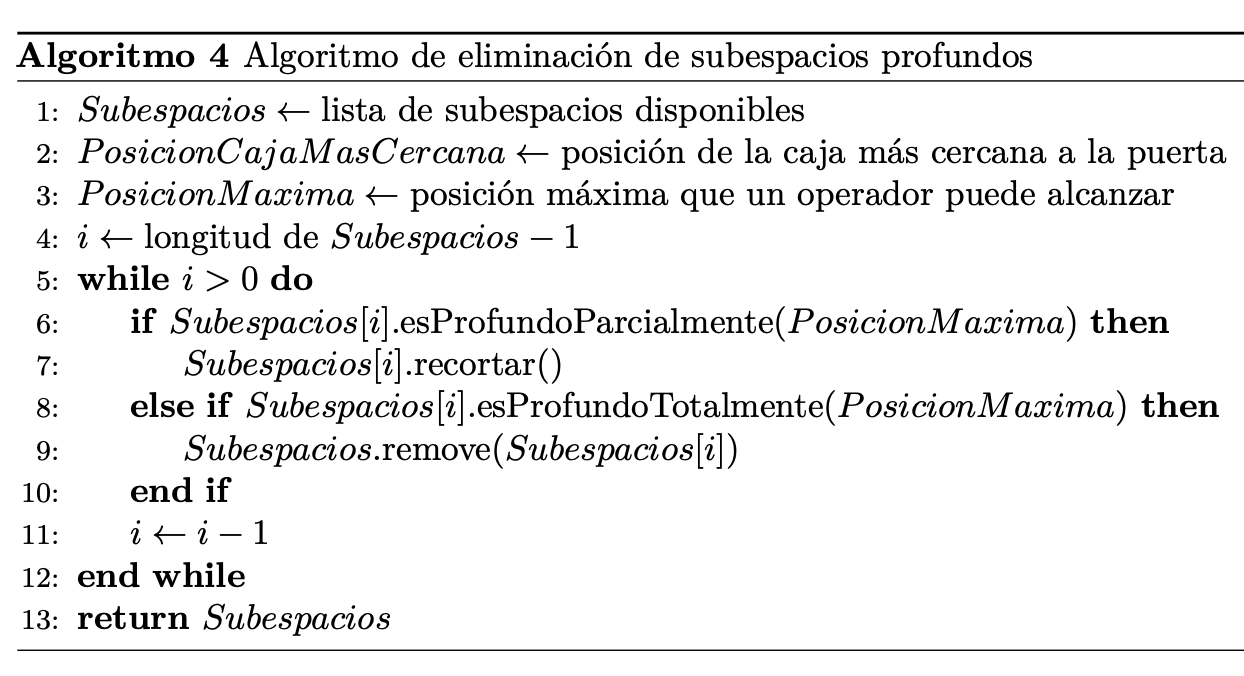
\includegraphics[width=0.48\textwidth]{pic/subespacios-profundos.png}
        \end{figure}
    \end{exampleblock}
\end{frame}

\begin{frame}{\href{https://raw.githubusercontent.com/josegustavo/lcp/main/lcp/presentation/pic/lcp.gif}{Ejemplo de Llenado Manual}}
    \begin{figure}
        \centering
        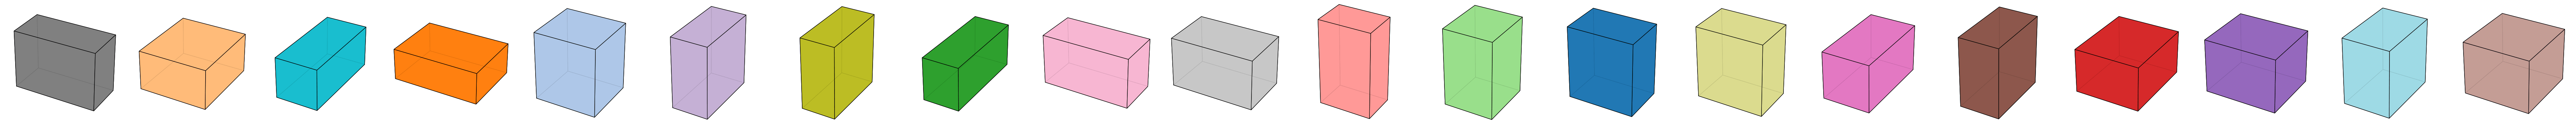
\includegraphics[width=.8\textwidth]{pic/cubos.png}
    \end{figure}
    \begin{figure}
        \centering
        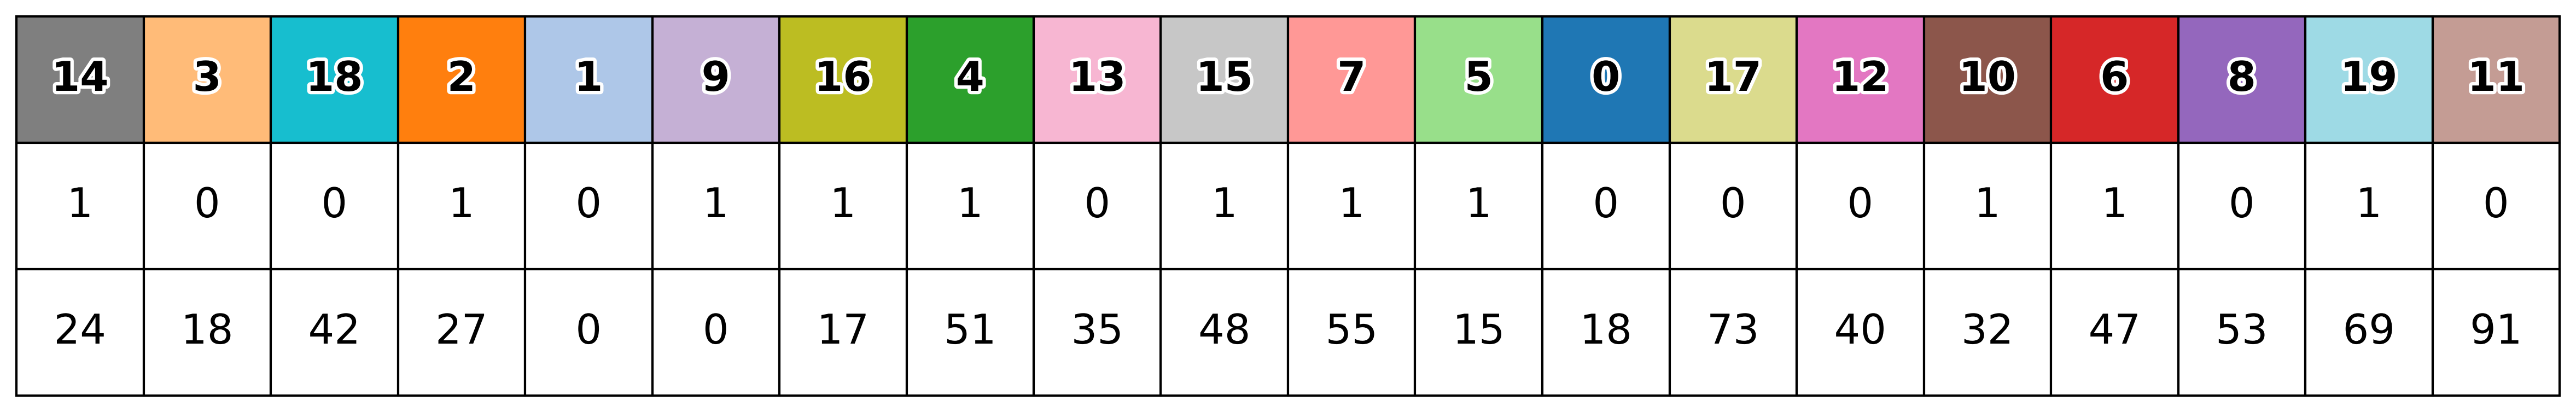
\includegraphics[width=.8\textwidth]{pic/tabla_colores_3x20.png}
    \end{figure}
    \begin{figure}
        \centering
        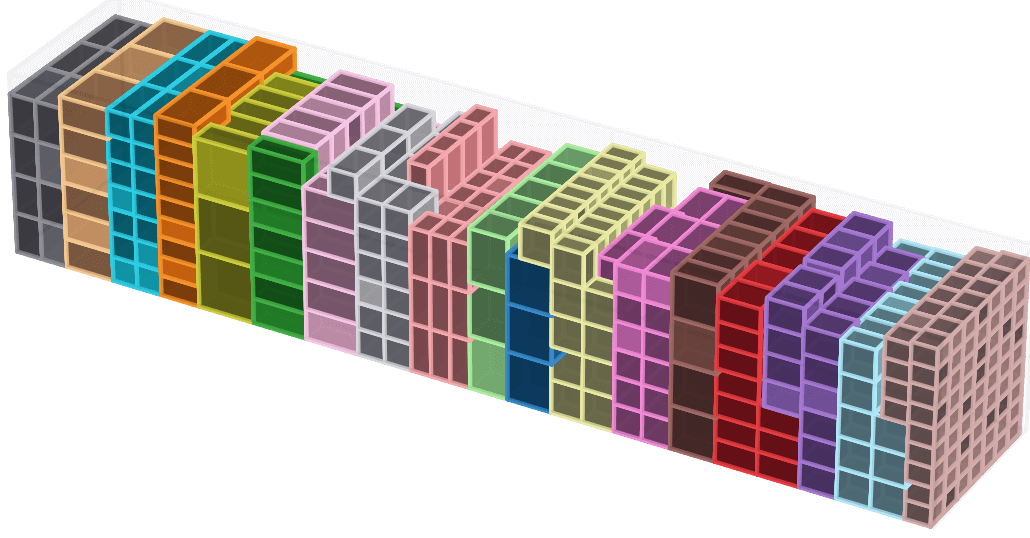
\includegraphics[width=.8\textwidth]{pic/contenedor-lleno.png}
    \end{figure}
\end{frame}

\begin{frame}{Algoritmo Genético: Pasos}
    \begin{enumerate}[<+-| alert@+>]
        \item Generación aleatoria de la población inicial
        \item Método de torneo binario para la selección
    \end{enumerate}
\end{frame}

\begin{frame}{Algoritmo Genético: Cruce}
    \begin{enumerate}[<+-| alert@+>]
        \setcounter{enumi}{2}
        \item Adaptación del operador de cruce de un punto
    \end{enumerate}
    \begin{figure}
        \centering
        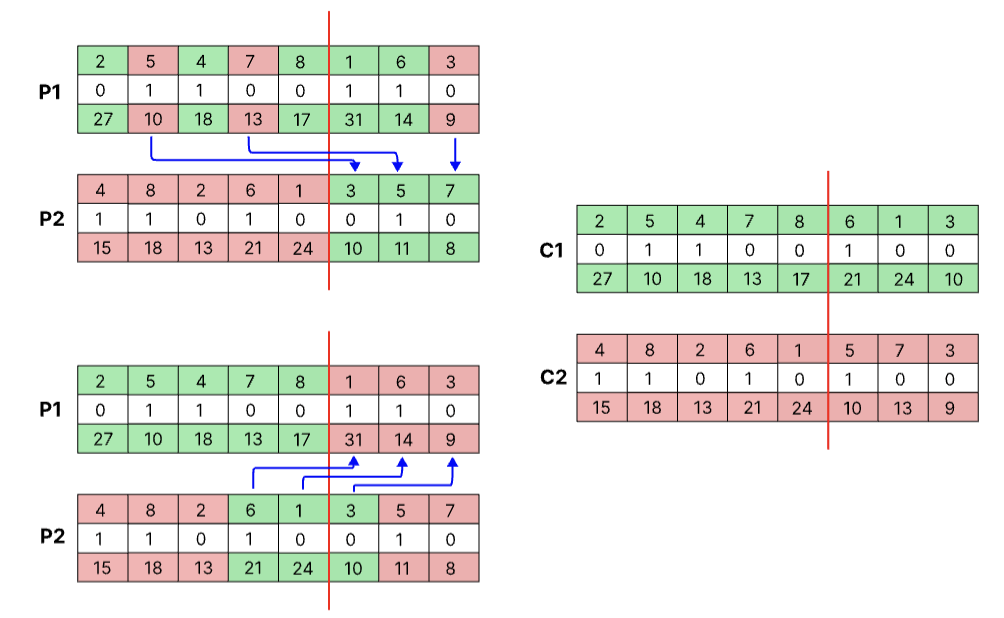
\includegraphics[width=.75\textwidth]{pic/ag-cruce.png}
        \caption*{Método de cruce adaptado para permutaciones\\
            que evita generar soluciones no factibles}
        \label{fig:solucion}
    \end{figure}
\end{frame}

\begin{frame}{Algoritmo Genético: Mutación}
    \begin{enumerate}[<+-| alert@+>]
        \setcounter{enumi}{3}
        \item Adaptación del operador de mutación de tres tipos
    \end{enumerate}
    \vspace{1cm}
    \begin{figure}[H]
        \centering
        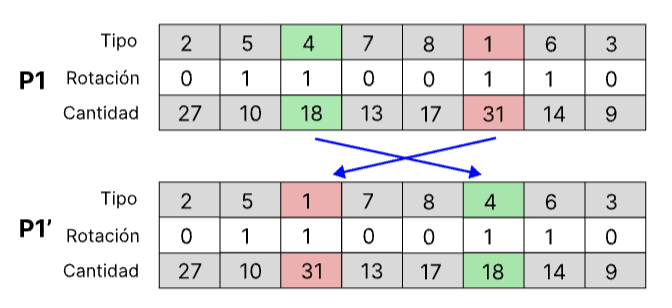
\includegraphics[width=0.35\textwidth]{pic/ag-mutacion1.png}
        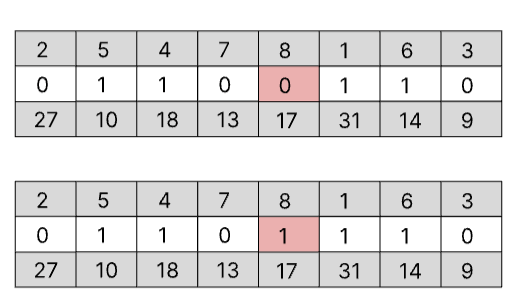
\includegraphics[width=0.275\textwidth]{pic/ag-mutacion2.png}
        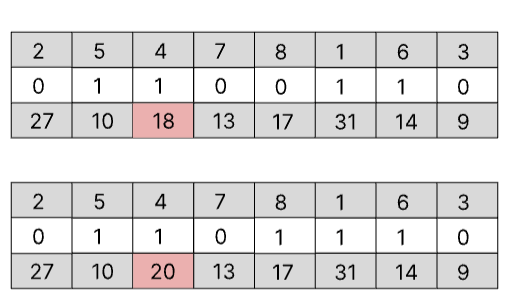
\includegraphics[width=0.275\textwidth]{pic/ag-mutacion3.png}
        \caption*{Métodos de mutación para \\
            el \textbf{orden}, la \textbf{rotación} y la \textbf{cantidad} por tipo}
    \end{figure}
\end{frame}

\begin{frame}{Diseño de procedimientos de mejora}
    \begin{columns}
        \begin{column}{0.6\textwidth}
            \begin{exampleblock}{Procedimiento de mejora de las soluciones}
                \begin{itemize}[<+-| alert@+>]
                    \item Ayuda a completar espacios vacíos si aún hay paquetes disponibles.
                    \item Aplicarla durante el llenado podría empeorar una solución.
                    \item Aplicarla luego del llenado garantiza que la solución no sea peor.
                    \item Agregan tiempo adicional de cómputo.
                \end{itemize}
            \end{exampleblock}
        \end{column}
        \begin{column}{0.4\textwidth}
            \begin{figure}
                \centering
                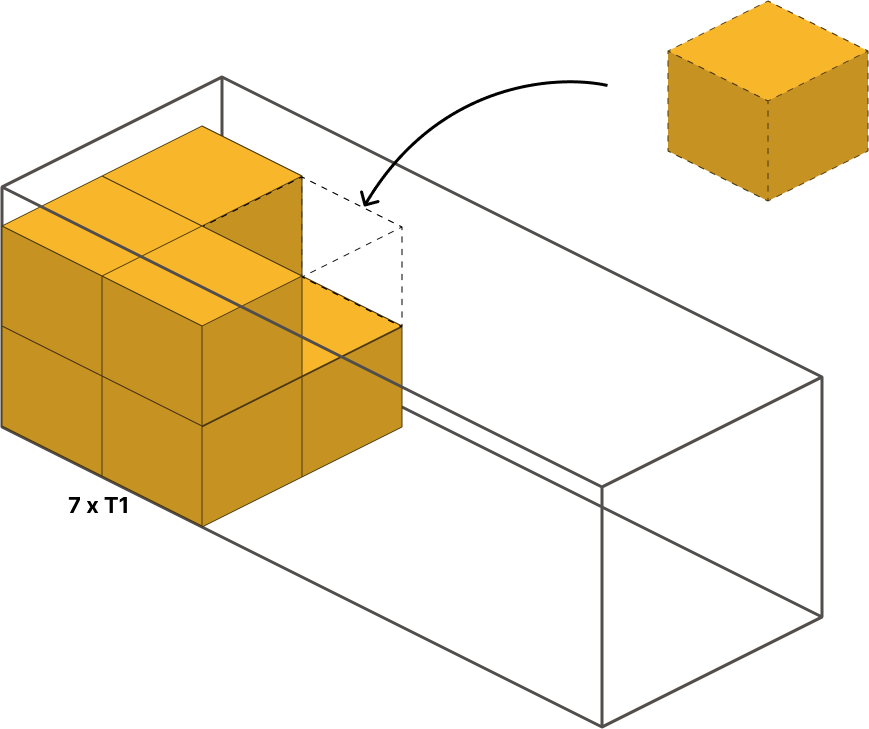
\includegraphics[width=0.85\textwidth]{pic/llenado_adicional_durante.png}
            \end{figure}
            \begin{figure}
                \centering
                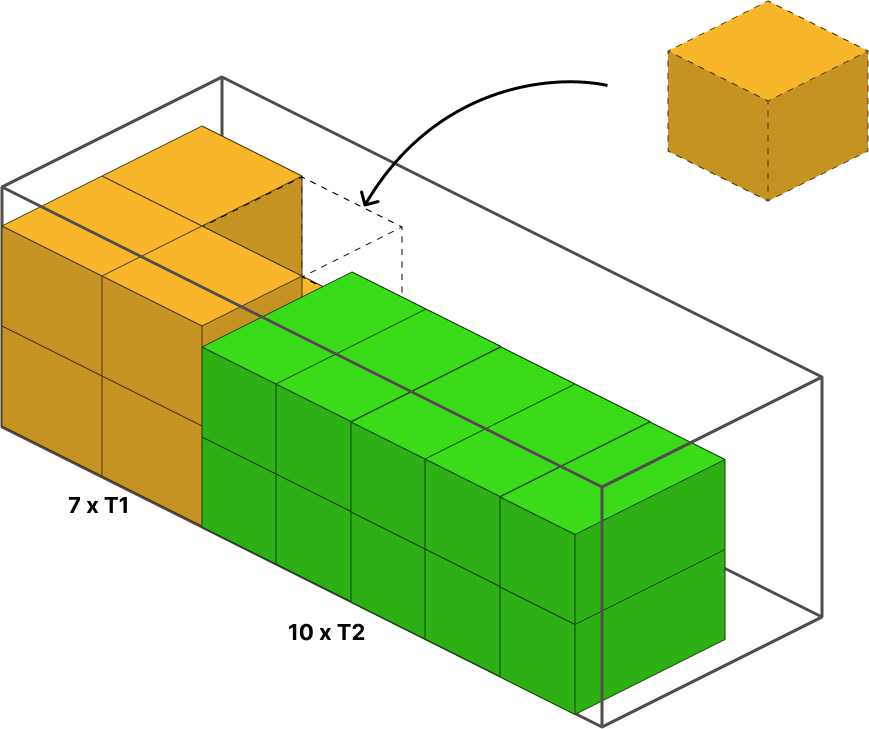
\includegraphics[width=0.85\textwidth]{pic/llenado_adicional_final.png}
            \end{figure}
        \end{column}
    \end{columns}
\end{frame}

\section[Experimentación]{Estudio Computacional}

\begin{frame}{Estudio Computacional}
    \begin{exampleblock}{Generación de Datos de Prueba}
        \begin{itemize}[<+-| alert@+>]
            \item Un contenedor con dimensiones fijas $12010 \times 2330 \times 2380 mm$.
            \item Instancias con $5$, $10$, $20$, $30$, $40$ y $50$ tipos de paquetes.
            \item Tamaños de paquetes aleatorios entre $250$ y $750$mm
            \item Asignación de beneficios aleatorios a cada paquete entre $10$ y $100$
        \end{itemize}
    \end{exampleblock}
\end{frame}

\begin{frame}{Estudio Computacional}
    \begin{exampleblock}{Configuración del Algoritmo}
        \begin{itemize}[<+-| alert@+>]
            \item Algoritmos implementados en Python 3.10.
            \item Población inicial de 100 individuos.
            \item $P_{cross}=0.8$.
            \item $P_{mut}=0.05$.
        \end{itemize}
    \end{exampleblock}
\end{frame}

\begin{frame}{Estudio Computacional}
    \begin{exampleblock}{Variantes del algoritmo}
        Comparar las distintas configuraciones del algoritmo
        \begin{itemize}[<+-| alert@+>]
            \item \textbf{M0}: Sin mejora del algoritmo en el llenado.
            \item \textbf{M1}: Llenado adicional durante a toda la población.
            \item \textbf{M2}: Llenado adicional al final a toda la población.
            \item \textbf{M3}: De tipo M2 pero aplicado al 50\% de la población.
            \item \textbf{M4}: De tipo M2, pero aplicado al mejor individuo de la población.
        \end{itemize}
    \end{exampleblock}
\end{frame}

\begin{frame}{Estudio Computacional}
    \begin{exampleblock}{Configuración del Experimento}
        \begin{itemize}[<+-| alert@+>]
            \item 25 problemas para cada tipo de instancia (5T, 10T, 20T, 30T, 40T y 50T), total 150 problemas.
            \item Tiempo fijo de 5 minutos para cada problema.
            \item Tiempo de ejecución total de 62.5 horas (2.6 días).
            \item Todas las variantes comienzan con la misma población inicial, para hacer una comparación justa.
        \end{itemize}
    \end{exampleblock}
\end{frame}

\begin{frame}{Estudio Computacional: Resultados}
    \begin{exampleblock}{Beneficio aportado por las soluciones}
        \begin{figure}
            \centering
            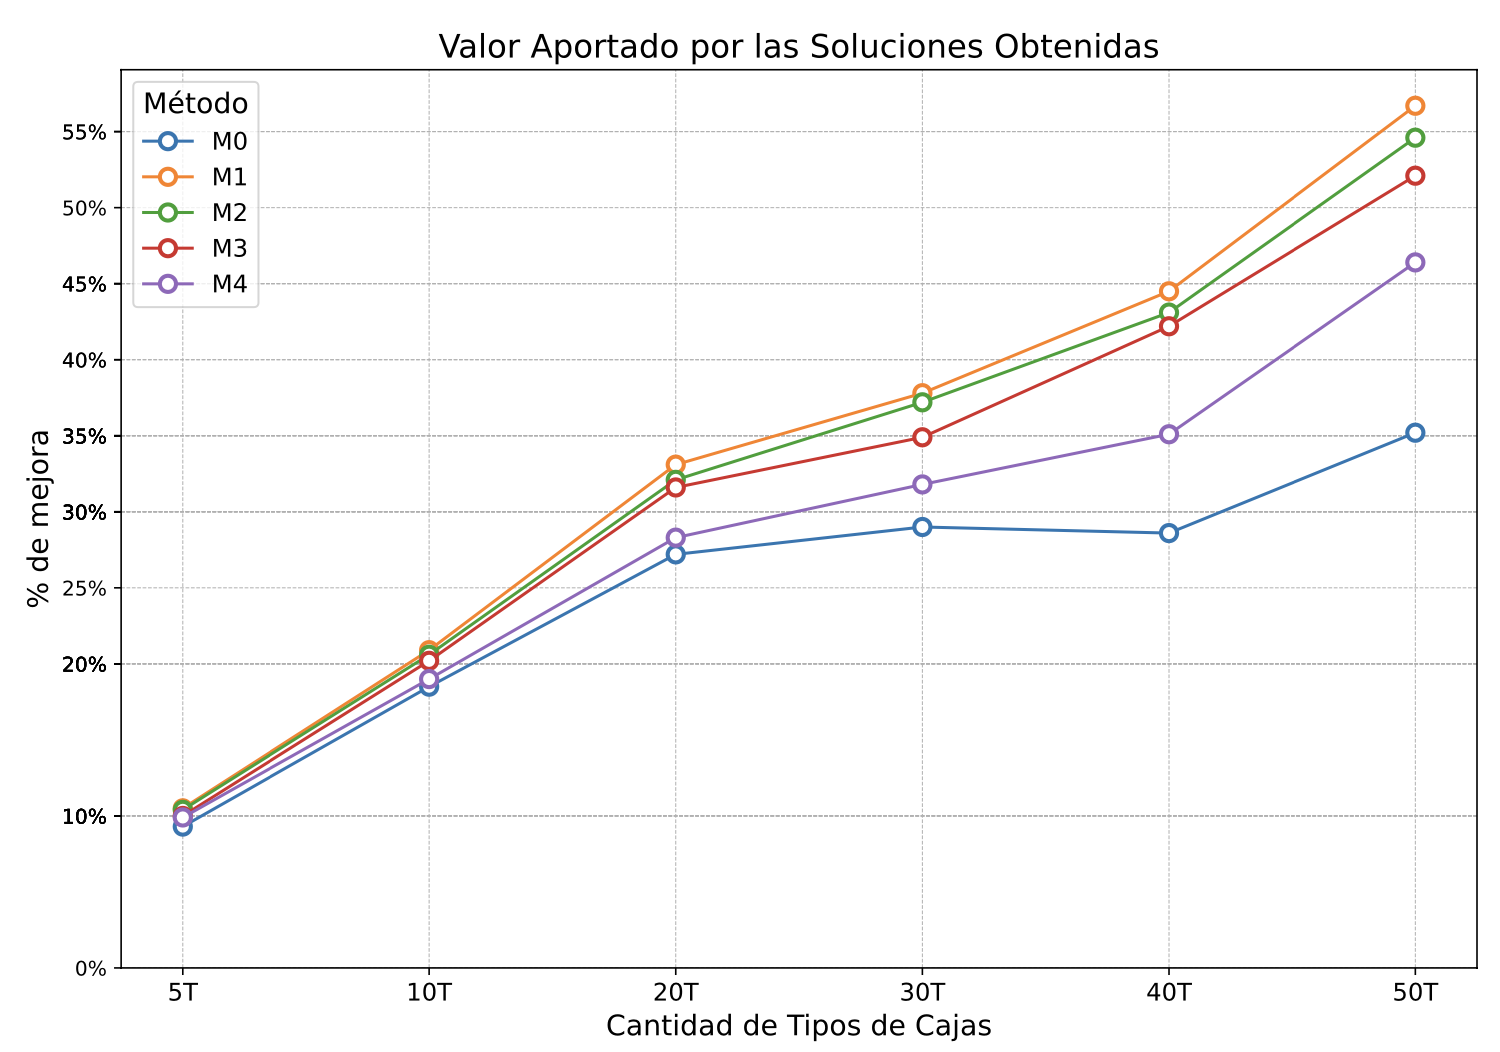
\includegraphics[width=0.8\linewidth]{pic/exp-valor-aportado.png}
            \label{fig:valor-aportado}
        \end{figure}
    \end{exampleblock}
\end{frame}

\begin{frame}{Estudio Computacional: Resultados}
    \begin{exampleblock}{Tiempo promedio en encontrar la mejor solución}
        \begin{figure}
            \centering
            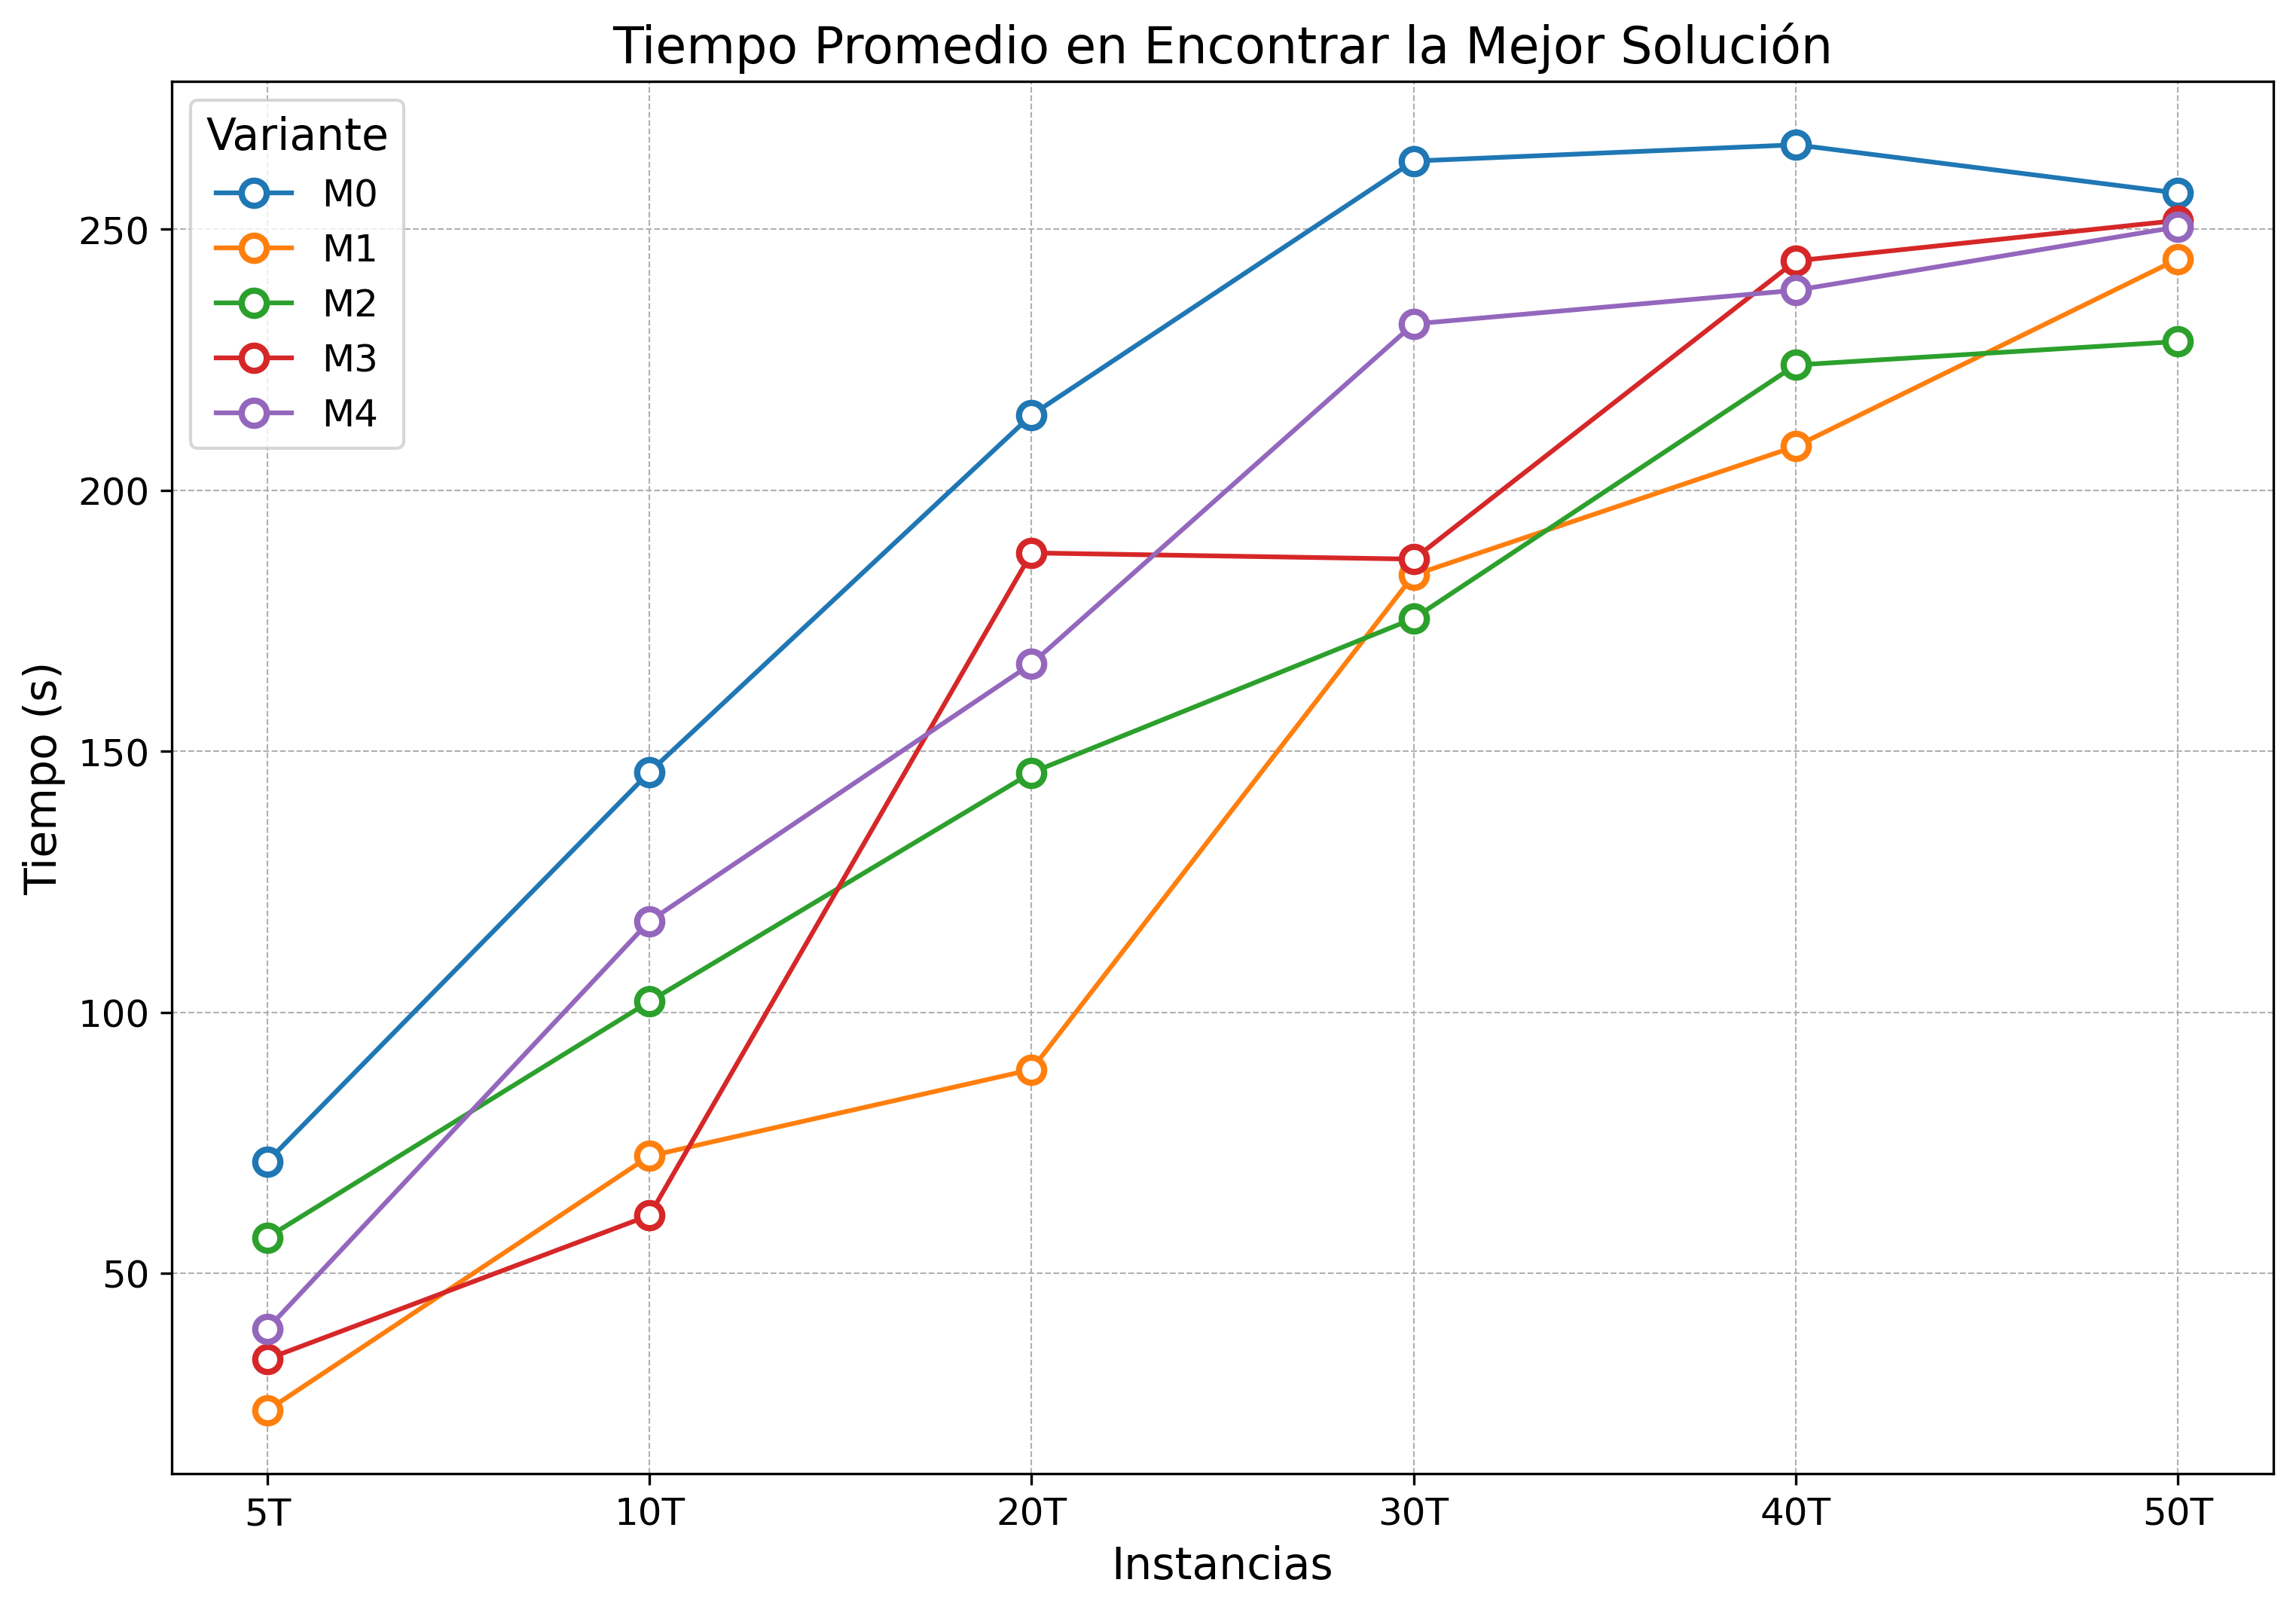
\includegraphics[width=0.8\linewidth]{pic/exp-tiempo-mejor-solucion.png}
            \label{fig:tiempo-mejor-solucion}
        \end{figure}
    \end{exampleblock}
\end{frame}

\begin{frame}{Estudio Computacional: Resultados}
    \begin{exampleblock}{Tiempo promedio por generación}
        \begin{figure}
            \centering
            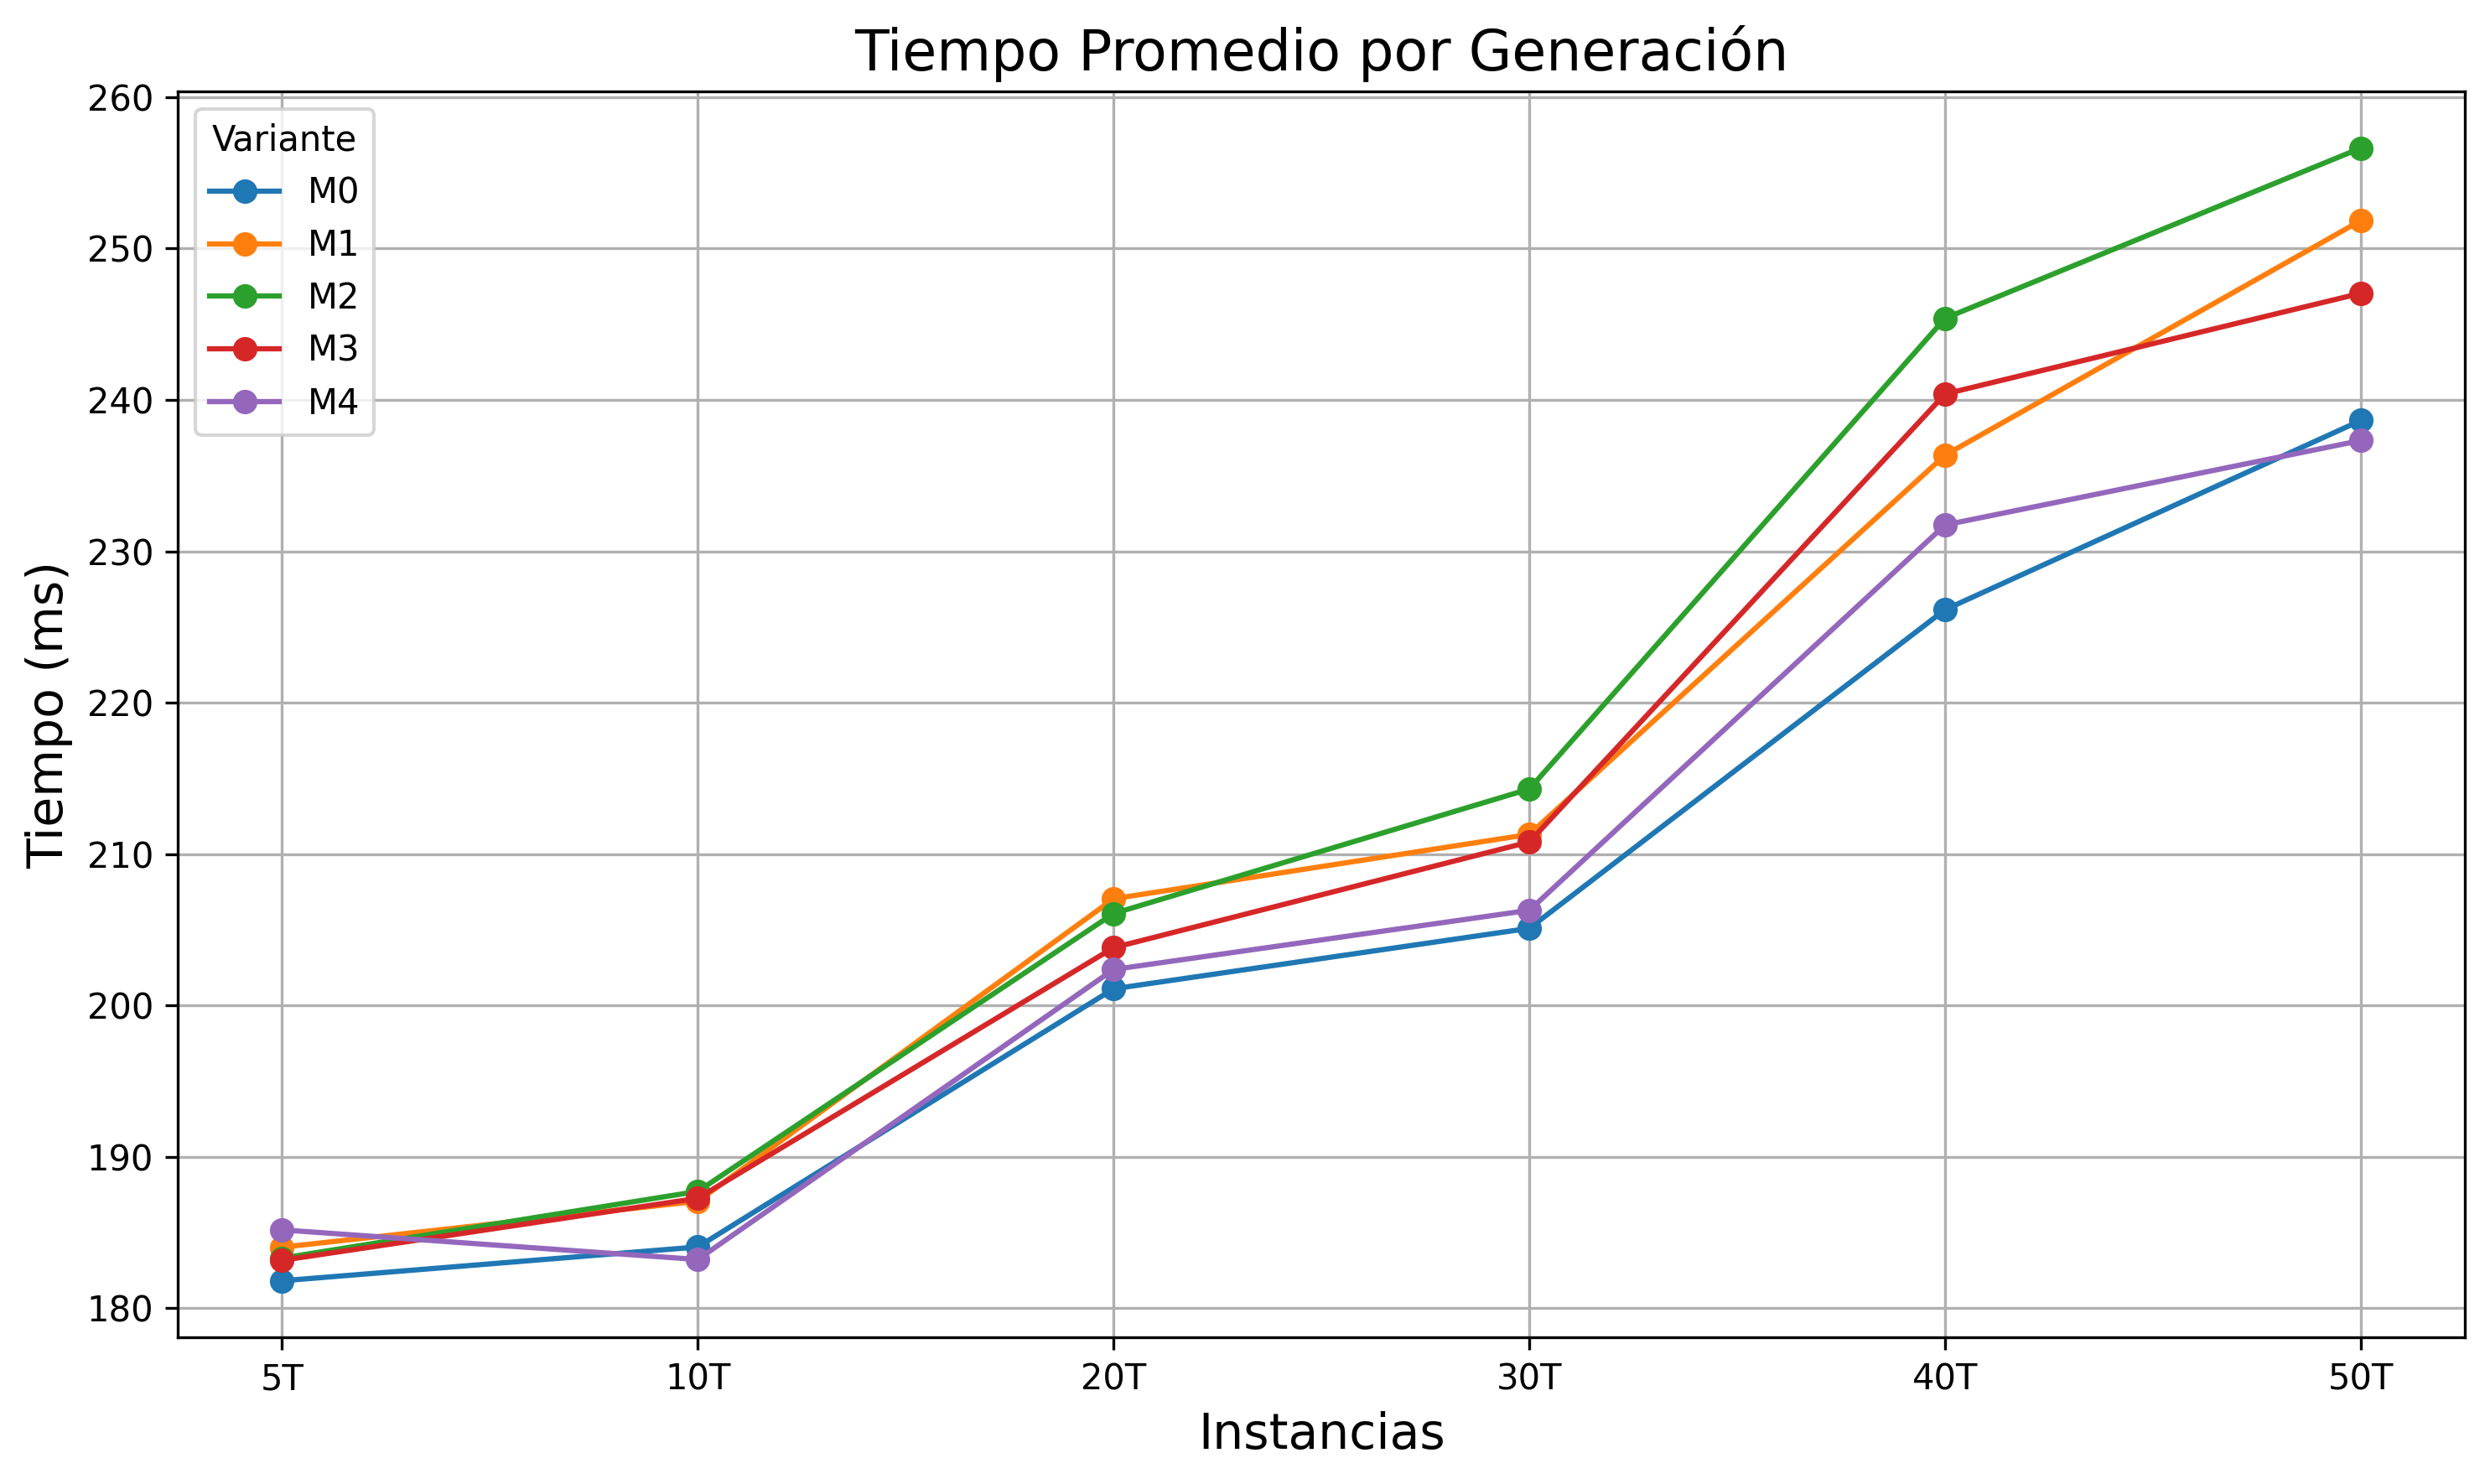
\includegraphics[width=0.8\linewidth]{pic/exp-tiempo-por-generacion.png}
        \end{figure}
    \end{exampleblock}
\end{frame}

\begin{frame}{Estudio Computacional: Resultados}
    \begin{exampleblock}{Rendimiento por método de mejora}
        \begin{figure}
            \centering
            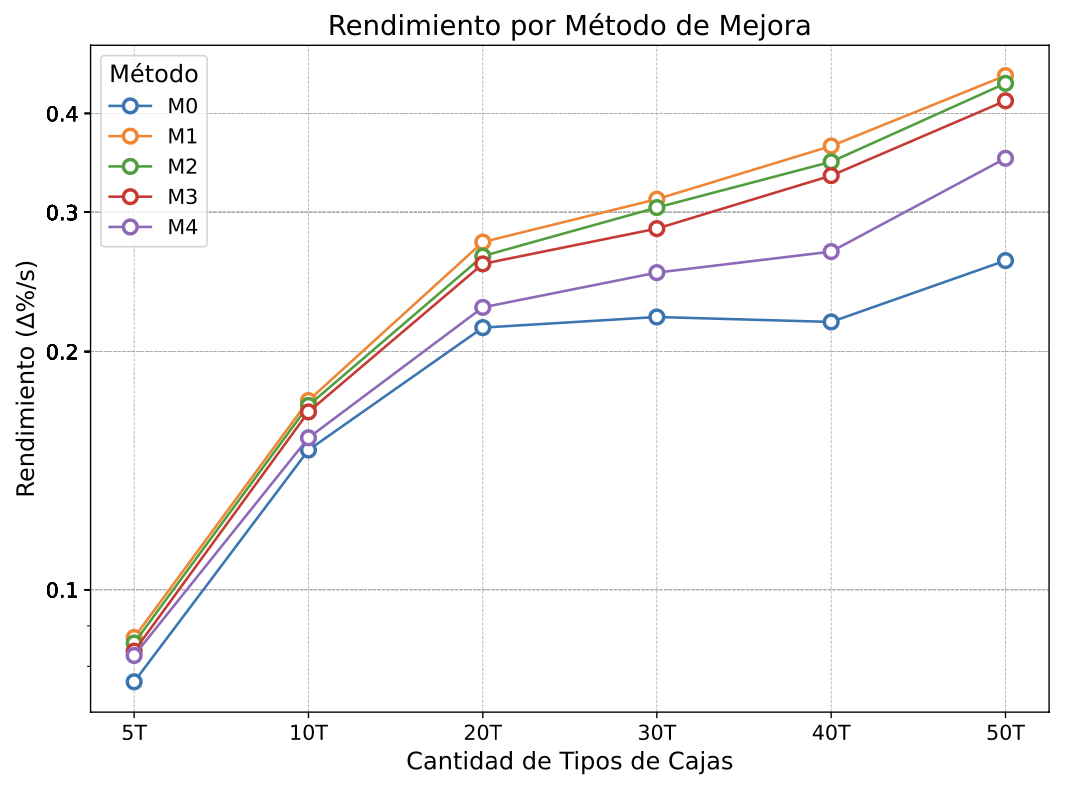
\includegraphics[width=0.8\linewidth]{pic/exp-rendimiento.png}
        \end{figure}
    \end{exampleblock}
\end{frame}

\begin{frame}{Estudio Computacional: Resultados}
    \begin{exampleblock}{Progreso de las soluciones del mejor método elegido: M1}
        \begin{figure}
            \centering
            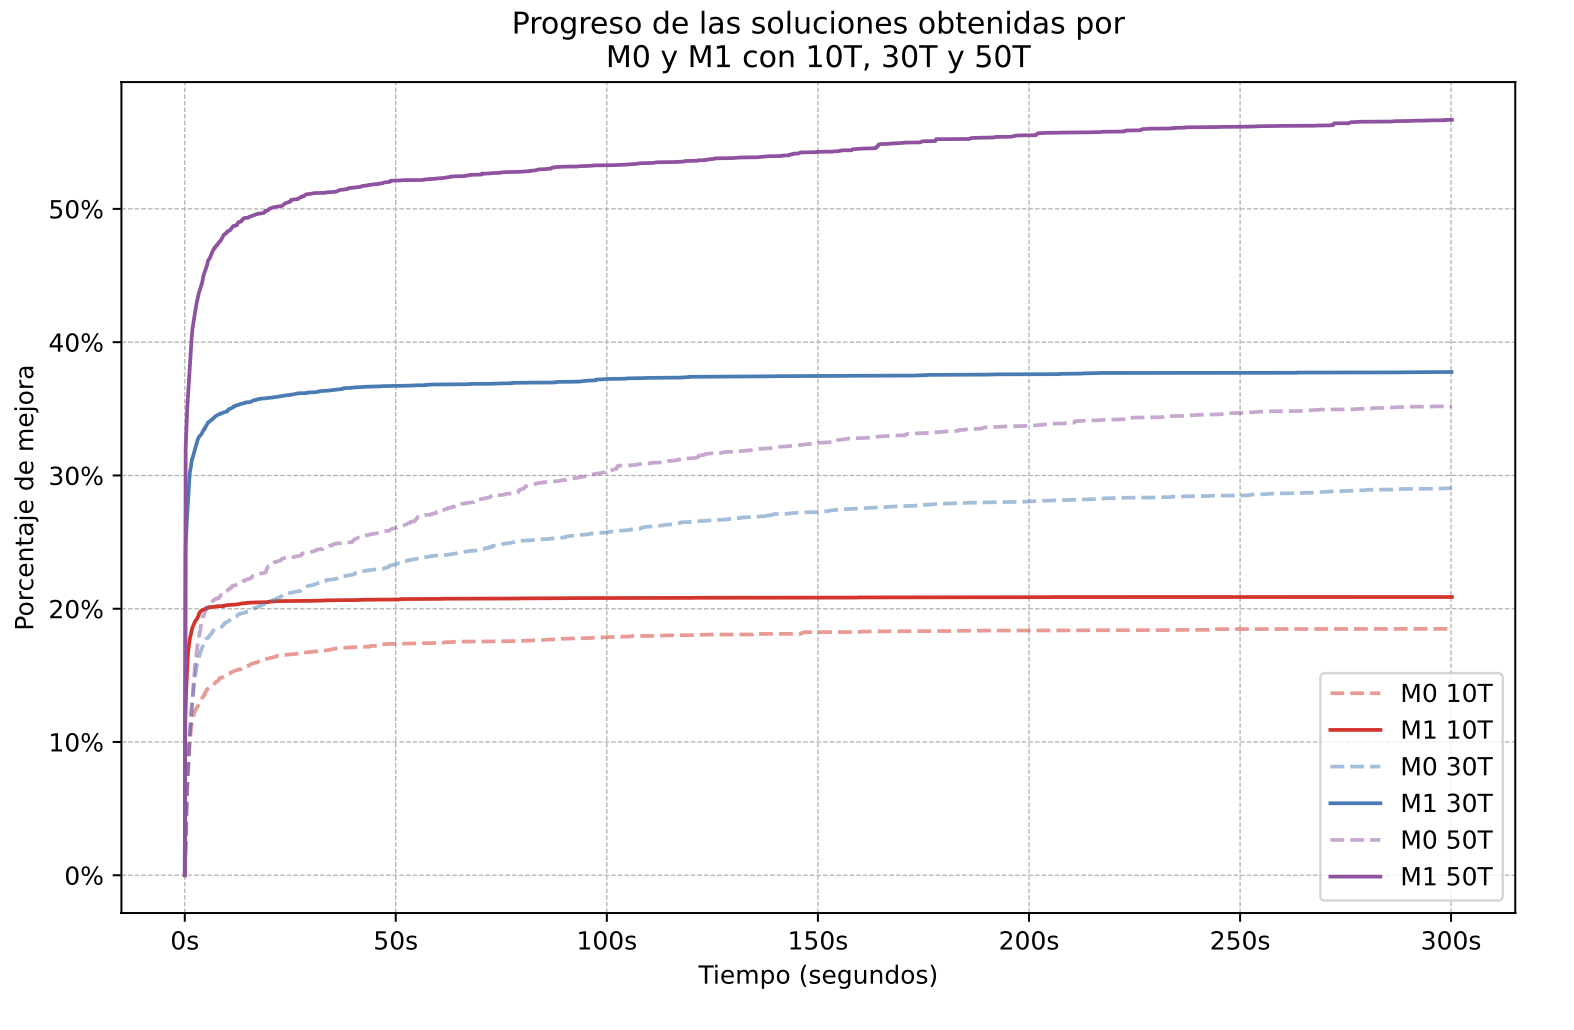
\includegraphics[width=0.8\linewidth]{pic/exp-progreso-soluciones.png}
        \end{figure}
    \end{exampleblock}
\end{frame}

\section[Conclusiones]{Conclusiones y Trabajos Futuros}

\begin{frame}{Conclusiones}
    \begin{itemize}[<+-| alert@+>]
        \item El algoritmo ha demostrado ser un método eficiente para determinar la disposición de los paquetes en el contenedor.
        \item Los métodos de mejoras consiguen reducir el tiempo necesario para encontrar la mejor solución.
        \item También consiguen mejorar la calidad de las soluciones.
        \item Elevado número de tipos de paquetes necesitan más tiempo para converger.
    \end{itemize}
\end{frame}

\begin{frame}{Trabajos Futuros}
    \begin{itemize}[<+-| alert@+>]
        \item Diseñar otros tipos de operadores de cruce y mutación.
        \item Considerar otras restricciones prácticas.
        \item Probar el algoritmo con datos reales.
        \item Incluir e  algoritmo en un DSS utilizado en tiempo real.
    \end{itemize}
\end{frame}

\begin{frame}
    \begin{center}
        {\Huge \textit{\fontfamily{pzc}\selectfont Gracias}}
    \end{center}
\end{frame}

\end{document}